\section{Ableitungen}

\subsection{Bedeutung von Ableitungen}

\subsection{Ableitungsregeln}

\subsubsection{Konstantenregel}

Die Ableitung einer Konstante ist 0 (und wird dann weggelassen).
Die Ableitung von $x$ ist 1.

\vspace*{-1.3cm}
\begin{align*}
    f(x) & = 3x + 5 \\
    f'(x) & = 3 \cdot 1 + 0
\end{align*}

\subsubsection{Differenz- und Summenregel}

Die Summanden einer Summe sowie Minuend und Subtrahend einer Subtraktion
werden unabhängig voneinander Abgeleitet.

\vspace*{-1.3cm}
\begin{align*}
    f(x) & = g(x) + u(x) & & f(x) = 5x + 2 \\
    f'(x) & = g'(x) + u'(x) & & f'(x) = 5 + 0\\
    f(x) & = g(x) - u(x) & & f(x) = 5x^2 - 5x + 3 \\
    f'(x) & = g'(x) +- u'(x) & & f'(x) = 10x - 5 + 0
\end{align*}

\subsubsection{Potenzregel und Faktorregel}

Die Potenzregel beschreibt, wie Potenzen abgeleitet werden. Dazu wird 1 vom
Exponenten subtrahiert (egal ob dieser positiv oder negativ ist) und der ursprügliche
exponent wird mit dem Term multipliziert. Faktoren im restlichen Term, z. B.
vor der Basis, bleiben generell unberührt (da es Multiplikation ist).

\vspace*{-0.5cm}
\begin{equation*}
    f(x) = x^n \qquad \Rightarrow \qquad
    f'(x) = n \cdot x^{n - 1}
\end{equation*}

\vspace*{-1cm}
\begin{align*}
    f(x) = x^3 \quad \Rightarrow \quad
    f'(x) = 3 \cdot x^2 \\
    f(x) = 2x^2 \quad \Rightarrow \quad
    f'(x) = 2 \cdot 2 \cdot x^1
\end{align*}

\subsubsection{Kettenregel}

Die Kettenregel hilft bem Ableiten, wenn sich die Funktion in eine innere und äußere Funktion
aufteilen lässt. Dies ist z. B. bei Potenzen, Sinusfunktion usw. der Fall.
Die Kettenregel besagt, dass die Ableitung einer zerlegbaren Funktion die Ableitung
der inneren Funktion multipliziert mit der Ableitung der äußeren Funktion ist.

\begin{equation*}
    f(x) = g(u(x)) \qquad \Rightarrow \qquad
    f'(x) = u'(x) \cdot g'(u(x)) \\
\end{equation*}
\vspace*{-0.5cm}
\begin{align*}
    & f(x) = (2x - 1)^3 \qquad & & i(x) = 2 \cdot e^{2x - 1} \qquad & & j(x) = \sin(2x) \\
    & f'(x) = 2 \cdot 3 \cdot (2x - 1)^2 \qquad & & i'(x) = -2 \cdot 2 \cdot e^{-2x - 1} \qquad & & j'(x) = 2 \cdot \cos(2x)
\end{align*}

\subsubsection{Produktregel}
Besteht eine Funktion aus 2 Termen, die multipliziert werden, so lässt sich die Produktregel
anwenden. Dadurch kann aufwendiges Ausmultiplizieren vermieden werden.

\begin{align*}
    f(x) = u(x) \cdot v(x) \qquad & \Rightarrow \qquad
    f'(x) = u'(x) \cdot v(x) + u(x) \cdot v'(x) \\
    f(x) = (2x + 3) \cdot (4x - 5) \qquad & \Rightarrow \qquad
    f'(x) = 2 \cdot (4x - 5) + (2x + 3) \cdot 4
\end{align*}


\subsubsection{Quotientenregel}

Die Quotientenregel ist ähnlich zur Produktregel und lässt sich für Divisionen von 2 als
Funktionen zu betrachtende Terme anwenden (der Nenner der Ableitung ist die Produktregel).

\begin{align*}
    f(x) = \frac{u(x)}{v(x)} \qquad & \Rightarrow \qquad f'(x) = \frac{u'(x) \cdot v(x) + u(x) \cdot v'(x)}{(v(x))^2} \\[15pt]
    f(x) = \frac{2x + 3}{4x - 5} \qquad & \Rightarrow \qquad f'(x) = \frac{2 \cdot (4x - 5) + (2x + 3) \cdot 4}{(4x - 5) \cdot (4x - 5)}
\end{align*}

\clearpage

\section{Kurvendiskussion}

\subsection{Nullstellen}

Die Nullstellen einer Funktion können durch Umformung, die pq-Formel bei quadratischen Funktionen oder
mit dem Taschenrechner gelöst werden (und Polynomdivision).
Bei der pq-Formel muss dazu zuerst der Vorfaktor $a$ durch Umformen entfernt werden
(gleich 1 sein). Wenn die Summe unter der Wurzel negativ ist, so gibt es keine Lösungen.

\begin{align*}
    & f(x) = x^2 + px +q \\[10pt]
    & x_{1,2} = -\frac{p}{2} \pm \sqrt{(\frac{p}{2})^2 - q}
\end{align*}

\subsection{Extrempunkte}

Globale Extrempunkte bezeichnen die höchsten bzw. tiefsten Punkte eines Graphen für den
gesamten Definitionsbereich. Lokale Extrempunkte bezeichnen diese höchsten oder tiefsten
Punkte in einem bestimmten Bereich.
Für eine Extremstelle der Funktion $f(x)$ gilt, dass die 1. Ableitung gleich 0 und die 2.
Ableitung ungleich 0 sein muss an dieser Stelle.
Ist die 2. Ableitung kleiner als 0, liegt ein Hochpunkt vor.
Ist die 2. Ableitung größer als 0, so liegt ein Tiefpunkt vor.

\begin{align*}
    & f'(x) = 0 \qquad und \qquad f''(x) \neq 0 \\
    & f''(x) < 0 \qquad \Rightarrow \qquad Hochpunkt \\
    & f''(x) > 0 \qquad \Rightarrow \qquad Tiefpunkt \\
\end{align*}

\subsection{Wendepunkte}

Wendepunkte einer Funktion liegen dann vor, wenn sich dass Vorzeichen der Steigung (1. Ableitung)
ändert. An diesen Punkten ändert sich dann auch dass Krümmungsverhalten des Graphen
(vgl. Links- anstatt Rechtskurve beim Auto).
Für einen Wendepunkt gilt, dass die 2. Ableitung gleich 0 ist und die 3. Ableitung ungleich 0.
Für einen Sattelpunkt gilt außerdem, dass die 1. Ableitung gleich 0 ist.

\begin{align*}
    & f''(x) = 0 \qquad und \qquad f'''(x) \neq 0 \\
    & f'(x) = 0 \qquad \Rightarrow \qquad Sattelpunkt \\
\end{align*}

\subsection{Symetrie}

Ein Graph ist Achsensymetrisch an der y-Achse, wenn der Funktionswert für $x$ unabhängig vom
Vorzeichen von x ist: $f(x) = f(-x)$.

Bei der Punktsymetrie am Ursprung gilt, dass es zu jedem Punkt (x | y) einen Punkt (-x | -y)
geben muss: $f(x) = -f(-x)$.

\subsection{Verhalten im Unendlichen}

Mit dem Limes lässt sich bestimmen, wie sich eine Funktion im Unendlichen verhält.
So lässt sich z. B. herausfinden, ob eine Funktion begrenzt wächst.
Für $x$ gegen $\infty$ oder $-\infty$ lässt sich so ein Wert bestimmen.

\begin{equation*}
    \lim_{x \to \infty} f(x) = L \qquad \qquad \lim_{x \to -\infty} f(x) = L
\end{equation*}

\subsection{Definitions und Wertebereich}

Der Definitionsbereich beschreibt alle Werte für $x$, denen bei einer Funktion $f(x)$
ein Wert für $y$ zugeordnet werden kann. Dies ist z. B. bei Wurzelfunktionen nicht
für negative Werte von $x$ möglich. Dabei können die mathematischen Zahlenbereich
genutzt werden sowie weitere Bedingungen bei Defintion der Defintionsmenge einer Funktion.
\newline

Der Wertebereich einer Funktion hingegen beschreibt den Bereich, in dem alle y-Werte
der Funktion liegen. Bei vielen Funktionen ist dieser Bereich $\mathbb{W}$ gleich $\mathbb{R}$,
aber z. B. für Wurzelfunktion liegen alle Werte nur in den positiven Zahlen. 

\begin{align*}
    & \mathbb{N} = \textnormal{natürliche} \qquad \mathbb{Z} = \textnormal{ganze} \qquad \mathbb{Q} = \textnormal{rationale} \qquad \mathbb{R} = \textnormal{reelle} \\
    & \qquad f(x) = x^3 \qquad \Rightarrow \qquad \mathbb{D} = \mathbb{R} \\
    & \qquad f(x) = x^2 \qquad \Rightarrow \qquad \mathbb{W} = \{ f(x) \in \mathbb{R} | f(x) \geq 0 \}
\end{align*}

\subsection{Monotonie und Krümmung}

Die Monotonie einer Funktion bezeichnet, ob die Funktion in einem bestimmten
Intervall nur steigt oder nur fällt (positive/negative Steigung).
Die zu bestimmenden Intervalle sind dabei zwischen allen Punkten, wo
sich die Steigung ändert, also zwischen allen Extremstellen und zwischen Extremstellen
und Unendlichkeit.

\begin{equation*}
    f'(x) > 0 \quad \Rightarrow \quad \textnormal{monoton steigent} \qquad f'(x) < 0 \quad \Rightarrow \quad \textnormal{monoton fallend}
\end{equation*}

Die Krümmung bezeichnet die Änderung der Steigung, also ob sich die Steigung um einen
positiven oder negativen Wert verändert. Die Krümmung muss dabei in den Intervallen zwischen
den Wendepunkten und denen zwischen Wendepunkten und Unendlichkeit bestimmt werden.

\begin{equation*}
    f''(x) > 0 \quad \Rightarrow \quad \textnormal{links gekruemmt} \qquad f''(x) < 0 \quad \Rightarrow \quad \textnormal{rechts gekruemmt}
\end{equation*}

\subsection{Tangentengleichung}

Für einen Punkt $P$ auf einem Graphen lässt sich eine Tangente $T$ an dieser Funktion $f$
konstruieren. Wenn $x_p$ und $y_p$ die Koordinaten von $P$ sind, so lässt sich
eine Tangente mithilfe der 1. Ableitung der Funktion wie folgt bilden.

\begin{equation*}
    T(x) = f'(x_p) \cdot (x - x_p) + y_p
\end{equation*}

\subsection{Normalengleichung}

Eine Normale einer Funktion $f$ ist eine Gerade die orthogonal (90° Winkel) zu einer Tangente
von $f$ im Punkt $P$ liegt. Die Normalengleichung ist dabei wie die Tangentengleichung, nur
dass die Steigung geändert wurde.

\begin{equation*}
    N(x) = -\frac{1}{f'(x_p)} \cdot (x - x_p) + y_p
\end{equation*}

\clearpage

\section{e-Funktion}

Die e-Funktion, benannt nach Euler, ist eine besondere Exponentialfunktion, die abgeleitet
sich selbst ergibt und die Umkehrfunktion des natürlichen Logarithmus ist.

Es gilt $e = 2.7 1828 1828 45 90 45 ...$

\begin{equation*}
    f(x) = e^x \qquad f'(x) = e^x \qquad f^{-1} = ln(x)
\end{equation*}

Jede Exponentialfunktion $x^a$ lässt sich außerdem mit e als Basis darstellen.

\begin{equation*}
    e(x) = a^x = e^{x \cdot ln(a)}
\end{equation*}

Der natürliche Logrithmus und die e-Funktion sind Umkehrfunktionen zueinander und heben
sich gegenseitig auf.

\begin{equation*}
    ln(e^x) = x = e^{ln(x)}
\end{equation*}

\section{Funktionsscharen}

Eine Funktionsschar besteht aus Funktionen, die sich nur durch den Wert des
Scharparameters $k$ unterscheiden. $f_1$ und $f_3$ sind beide Teil der Funktionsschar
$f$.

\begin{equation*}
    f_k(x) = k \cdot x^3 - 2x^2 \qquad f_1(x) = 1 \cdot x^3 - 2x^2 \qquad f_3(x) = 3 \cdot x^3 - 2x^2
\end{equation*}

Bildet man die Ableitungen, so bleibt der Scharparameter erhalten.

\begin{equation*}
    f'_{k}(x) = k \cdot 3x^2 - 4x^1 \qquad f''_{k}(x) = k \cdot 6x - 4 \qquad f'''_{k}(x) = k \cdot 6
\end{equation*}

Auch beim gleichsetzen mit $0$ sind einige Nullstellen weiterhin abhängig vom Scharparameter.
Diese Nullstellen lassen sich nach $k$ umformen, sodass man $k$ in Abhängigkeit von $x$ erhält.
Ersetzt man $k$ durch diesen neuen Term mit $x$, so erhält man eine neue Funktion (Ortlinie).
Diese beschreibt für eine Nullstelle alle Orte, wo die Scharfunktionen mit $k$ diese
bestimmte Nullstelle haben.

\begin{equation*}
    f'_k(x) = 0 \qquad x_1 = 0, \quad x_2 = \frac{4}{3k} \quad \Rightarrow \quad k = \frac{4}{3x} \quad \Rightarrow \quad ex(x) = \frac{4}{3x} \cdot x^3 - 2x^2
\end{equation*}

Die Funktion $ex(x)$ beschreibt alle Orte, wo die 1. Ableitung von $f$ gleich $0$ ist.
Somit beschreibt $ex(x)$ alle Minima (Extrempunkt), die bei $f$ für unterschiedliche $k$ entstehen können.

\begin{center}
    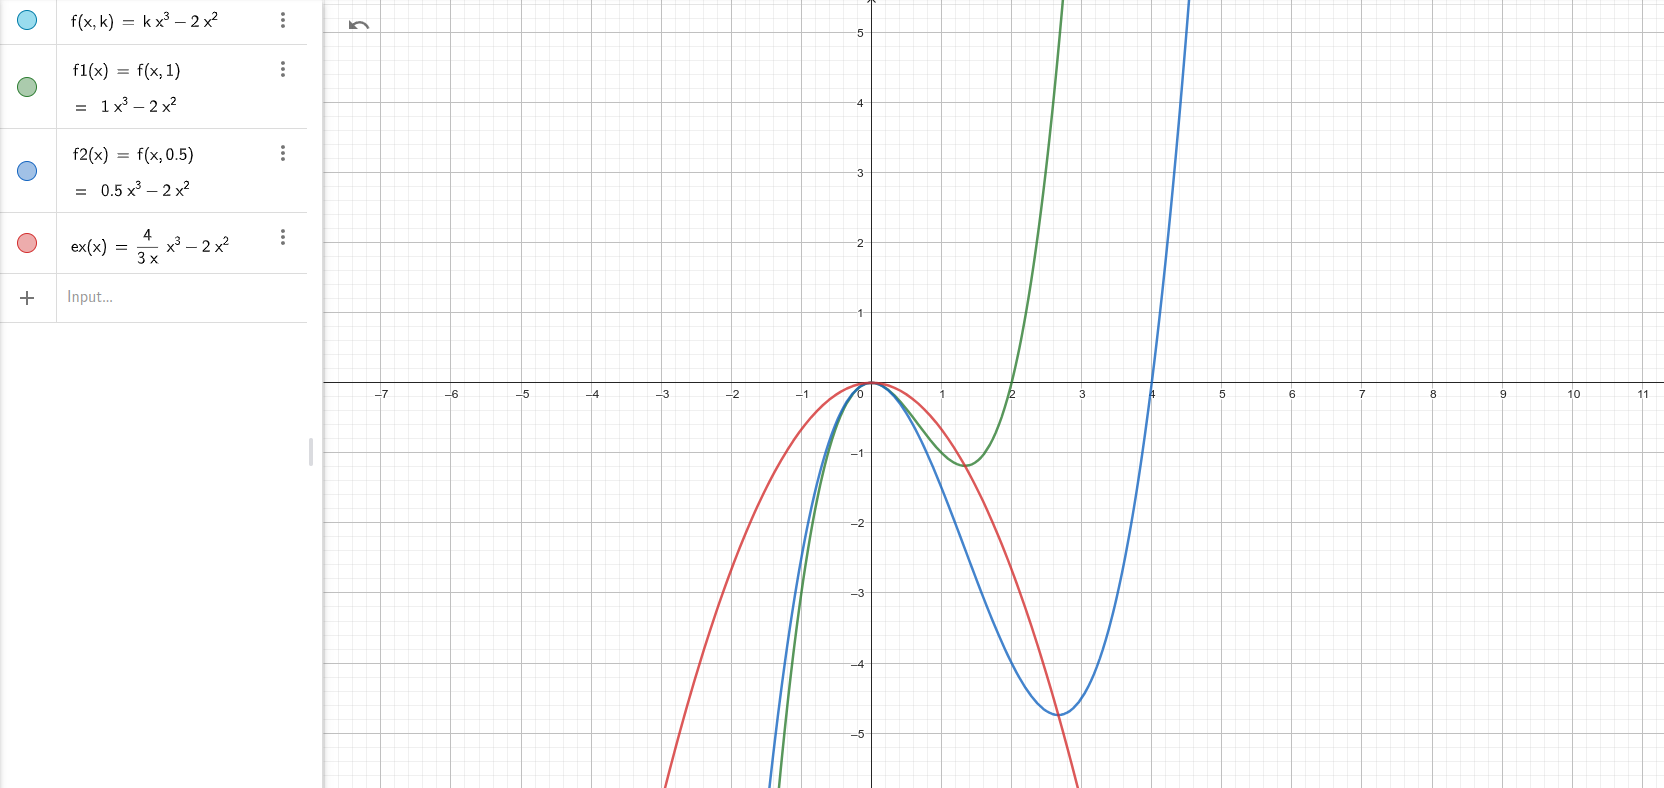
\includegraphics[width=1.0\textwidth]{images/2d-f-schar-example.png}
\end{center}

\clearpage

\section{Wachstum und Differentialgleichungen}

exponentielle wachstum
Differentialgleichungen dazu
begrenztes Wachstum
Differentialgleichungen dazu
logistisches Wachstum
Differentialgleichungen dazu

\section{Integrale und Flächen}

integrale -> idee der produktsummen zur unendlichkeit
stammfunktion bestimmten -> bestandsidee
flächeninhalte berechnen
rotationsvolumen
offene flächen
x > 0

\section{GTR Todo}

\section{Gauß Algorithmus}

gauß algorithmus

rref
